$l$ and $m$ are two parallel lines intersected by another pair of parallel lines $p$ and $q (\figref{fig:9.7.1.4})$,show that $\triangle ABC \cong \triangle CDA$.

\textbf{Figure :}
\begin{figure}[H]
    \centering
	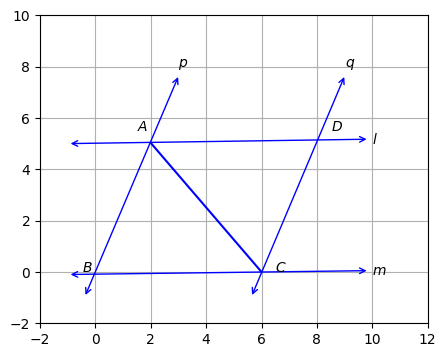
\includegraphics[width=\columnwidth]{chapters/9/7/1/4/fig/em1.png}
    \caption{Required parallelogram}
    \label{fig:9.7.1.4}
\end{figure}

\textbf{Solution :}
\begin{table}[H]
    \centering
      \begin{tabular}{|c|c|c|}
    \hline
        \textbf{Symbol} &\textbf{Description}&\textbf{Value}  \\
        \hline
        $\vec{B}$&Vertex at origin&$\vec{0}$\\
        \hline
        $a$ & Side of the parallelogram,$BC=DA$ & 6\\
        \hline
        $b$ & Side of the parallelogram,$AB=CD$& $\sqrt{29}$\\
        \hline
        $\theta$ & Angle of the parallelogram, $\angle ABC$& $\sin^{-1}\brak{{\frac{5}{\sqrt{29}}}}$\\
        \hline
    \end{tabular}

    \caption{Table of input parameters}
    \label{tab:9.7.1.4.1}
\end{table}

\begin{table}[H]
    \centering
       \begin{tabular}{|c|c|c|}
    \hline
        \textbf{Symbol} &\textbf{Description}&\textbf{Value}  \\
        \hline
	   $\vec{C}$&Vertex of parallelogram &$a\vec{e_1}$\\
        \hline
         $\vec{A}$&Vertex of parallelogram &$b\begin{pmatrix}
             \cos{\theta}\\
             \sin{\theta}
         \end{pmatrix}$\\
        \hline
        $\vec{D}$&Vertex of parallelogram &$\vec{C+A}$\\
        \hline
    \end{tabular}

    \caption{Table of output parameters}
    \label{tab:9.7.1.4.2}
\end{table}  
So,$\triangle ABC \cong \triangle CDA.\brak{by A-A-S}\brak{proved}$
